\documentclass[a4paper,12pt]{article}

% Кодировки и языковые настройки
\usepackage[utf8]{inputenc}
\usepackage[T2A]{fontenc}
\usepackage[english, russian]{babel}

% Разметка страницы
\usepackage[left=2cm, right=2cm, top=2cm, bottom=2cm]{geometry}

% Работа с графикой
\usepackage{graphicx}
\usepackage{float}
\usepackage{wrapfig}
\usepackage{tikz}

% Математические пакеты
\usepackage{amsmath, amsfonts, amssymb}

% Гиперссылки
\usepackage{hyperref}
\hypersetup{pdfborder=0 0 0, pdfstartview=FitH, linkcolor=blue, urlcolor=blue, colorlinks=true}

% Оформление заголовков и страниц
\usepackage{fancybox, fancyhdr}
\pagestyle{fancy}
\fancyhf{}
\fancyhead[L]{Задачи №2025, 1005, 1155}
\fancyhead[R]{Сайфуллин Д.Р., АиСД R23 1.3}
\fancyfoot[C]{\thepage}
\headsep=8mm
\footskip=8mm
\setlength{\parindent}{0mm}

% Цвета
\usepackage{xcolor}
\definecolor{urlcolor}{HTML}{3454D1}
\definecolor{linkcolor}{HTML}{3454D1}

% Листинги кода
\usepackage{listings}
\lstdefinestyle{codestyle}{
    backgroundcolor=\color{gray!10},
    commentstyle=\color{green!50!black},
    keywordstyle=\color{blue!80!black},
    stringstyle=\color{red!50!black},
    numberstyle=\tiny\color{gray},
    basicstyle=\ttfamily\footnotesize,
    breaklines=true,
    captionpos=b,
    numbers=left,
    numbersep=5pt,
    showstringspaces=false,
    tabsize=2
}
\lstset{style=codestyle}

% Создание обрамленных блоков
\usepackage{mdframed}
\newmdenv[
  leftmargin = 0.5em,
  skipabove = 0.5em,
  skipbelow = 0.5em,
  linewidth = 1pt,
  rightline = false,
  topline = false,
  bottomline = false
]{quotebox}

% Оглавление и заголовки
\newcommand{\addsection}[1]{
    \phantomsection
    \addcontentsline{toc}{section}{#1}
    \section*{\centering #1}
}

\newcommand{\addsubsection}[1]{
    \phantomsection
    \addcontentsline{toc}{subsection}{#1}
    \subsection*{\centering #1}
}

\begin{document}

% Титульный лист
\begin{titlepage}
    \centering
    {\large Федеральное государственное автономное образовательное учреждение\par}
    {\large высшего образования\par}
    {\bfseries САНКТ-ПЕТЕРБУРГСКИЙ НАЦИОНАЛЬНЫЙ ИССЛЕДОВАТЕЛЬСКИЙ УНИВЕРСИТЕТ ИТМО\par}
    {\bfseries Факультет систем управления и робототехники\par}
    \vfill
    {\Large \bfseries Лабораторная работа №1\par}
    {\Large \bfseries Задачи №2025, 1005, 1155\par}
    \vfill
    
    \begin{flushright}
        Студент: Сайфуллин Д.Р. \\
        Поток: АиСД R23 1.3 \\
        Преподаватель: Тропченко А.А.
    \end{flushright}
    \vfill
    Санкт-Петербург \\
    2025 г.
\end{titlepage}

\addsection{\href{https://acm.timus.ru/problem.aspx?space=1&num=2025}{Задача №2025. Стенка на стенку}}
Бокс, каратэ, самбо… Классические боевые единоборства пресытили аудиторию. Поэтому известный спортивный канал запускает новый формат соревнований, основанный на традиционной русской забаве — боях стенка на стенку.
В соревновании могут участвовать от двух до k команд, каждая из которых будет соперничать с остальными. Всего в соревновании примут участие n бойцов. Перед началом боя они должны разделиться на команды, каждый боец должен войти ровно в одну команду. За время боя два бойца сразятся, если они состоят в разных командах. Организаторы считают, что популярность соревнований будет тем выше, чем больше будет количество схваток между бойцами. Помогите распределить бойцов по командам так, чтобы максимизировать количество схваток между бойцами, и выведите это количество.\\[1em]
\textbf{Исходные данные:}
\begin{quotebox}
    В первой строке дано количество тестов $T$ $(1 \leq T \leq 10)$. В следующих $T$ строках перечислены тесты. В каждой из них записаны целые числа $n$ и $k$ через пробел $(2 \leq k \leq n \leq 10^4)$.
\end{quotebox}
\textbf{Результат:}
\begin{quotebox}
    Для каждого теста в отдельной строке выведите одно целое число --- ответ на задачу.
\end{quotebox}
\addsubsection{Рабочий код}
\begin{lstlisting}[language=python]
T = int(input())

for t in range(T):
    n, k = map(int, input().split())
    comm = [0] * k

    for j in range(k):
        comm[j] = n // k

    for j in range(n % k):
        comm[j] += 1

    res = 0
    for j in range(k-1):
        res += comm[j] * (n - comm[j])
        n -= comm[j]

    print(res)
\end{lstlisting}
\addsubsection{Объяснение алгоритма}
Для максимизации числа схваток между бойцами из разных команд, важно, чтобы количество бойцов в каждой из двух команд было максимально равным. Поэтому:
\begin{itemize}
    \item Распределяем n бойцов по k командам с использованием "остатков": определяем базовое количество бойцов в каждой команде как n//k. Остаток n\%k равномерно распределяется по k командам, чтобы часть команд содержала на 1 бойца больше.
    \item Считаем число возможных схваток: число схваток определяется как произведение количества бойцов из двух разных команд. Это эквивалентно подсчету всех возможных пар бойцов из разных команд.
\end{itemize}

\addsection{\href{https://acm.timus.ru/problem.aspx?space=1&num=1005}{Задача №1005. Куча камней}}
У вас есть несколько камней известного веса $w_1, \dots, w_n$. Напишите программу, которая распределит камни в две кучи так, что разность весов этих двух куч будет минимальной.\\[1em]
\textbf{Исходные данные:}
\begin{quotebox}
    Ввод содержит количество камней $n$ $(1 \leq n \leq 20)$ и веса камней $w_1, \dots, w_n$ $(1 \leq w_i \leq 100 000)$ --- целые, разделённые пробельными символами.
\end{quotebox}
\textbf{Результат:}
\begin{quotebox}
    Ваша программа должна вывести одно число --- минимальную разность весов двух куч.
\end{quotebox}
\addsubsection{Рабочий код}
\begin{lstlisting}[language=python]
def f(size, lst, i=0, sum1=0, sum2=0, min_=float('inf')):
    if i == size:
        return min(min_, abs(sum1 - sum2))
    min_ = f(size, lst, i + 1, sum1 + lst[i], sum2, min_)
    min_ = f(size, lst, i + 1, sum1, sum2 + lst[i], min_)
    return min_

if __name__ == '__main__':
    n = int(input())
    rocks = [int(w) for w in input().split()]
    print(f(n, rocks))
\end{lstlisting}
\addsubsection{Объяснение алгоритма}
Этот код решает задачу распределения камней в две кучи так, чтобы разность весов этих куч была минимальной. В начале программы считывается количество камней и их веса. Затем программа вызывает рекурсивную функцию \verb|search|, которая перебирает все возможные варианты распределения камней в две кучи и находит минимальную разность весов этих куч. Функция \verb|search| принимает массив камней, его размер, индекс текущего камня, сумму весов камней в первой куче и сумму весов камней во второй куче. Если индекс текущего камня равен размеру массива, функция вычисляет разность весов куч и обновляет минимальное значение разности. В противном случае функция вызывает себя дважды: с текущим камнем в первой куче и с текущим камнем во второй куче. Функция возвращает минимальное значение разности весов куч. В конце программы выводится минимальное значение разности весов куч. Этот код решает задачу за $O(2^n)$ времени, где $n$ --- количество камней.

\addsection{\href{https://acm.timus.ru/problem.aspx?space=1&num=1155}{Задача №1155. Дуоны}}
С развитием техники физики находят всё новые и новые элементарные частицы, с непонятными и даже загадочными свойствами. Многие слышали про мюоны, глюоны, странные кварки и прочую нечисть. Недавно были обнаружены элементарные частицы дуоны. Эти частицы названы так потому, что учёным удаётся создавать или аннигилировать их только парами. Кстати, от дуонов одни неприятности, поэтому от них стараются избавляться до начала экспериментов. Помогите физикам избавиться от дуонов в их установке.\\[0.5em]
Экспериментальная установка состоит из восьми камер, которые расположены в вершинах куба. Камеры промаркированы латинскими буквами A, B, C, …, H. Технически возможно создать, или наоборот, аннигилировать, два дуона, находящихся в смежных камерах. Вам нужно автоматизировать процесс удаления дуонов из установки.\\[1em]
\textbf{Исходные данные:}
\begin{quotebox}
    В единственной строке даны восемь целых чисел в пределах от 0 до 100, описывающих количество дуонов в камерах установки (сначала в камере A, потом в B, и т.д.).
\end{quotebox}
\textbf{Результат:}
\begin{quotebox}
    Выведите последовательность действий для удаления всех дуонов или слово «IMPOSSIBLE», если это невозможно. Каждое действие должно быть описано в отдельной строке, в следующем формате: маркер первой камеры, маркер второй (смежной с первой), далее плюс либо минус (создать или аннигилировать пару дуонов). Количество действий в последовательности не должно превосходить 1000.
\end{quotebox}
\addsubsection{Рабочий код}
\begin{lstlisting}[language=python]
import sys


def minus_p(x, y):
    x["n"] -= 1
    y["n"] -= 1
    print(f"{y['ch']}{x['ch']}-")


def plus_p(x, y):
    x["n"] += 1
    y["n"] += 1
    print(f"{y['ch']}{x['ch']}+")


def main():
    data = list(map(int, sys.stdin.read().split()))
    if len(data) < 8:
        print("IMPOSSIBLE")
        return

    a = {"ch": "A", "n": data[0]}
    b = {"ch": "B", "n": data[1]}
    c = {"ch": "C", "n": data[2]}
    d = {"ch": "D", "n": data[3]}
    e = {"ch": "E", "n": data[4]}
    f = {"ch": "F", "n": data[5]}
    g = {"ch": "G", "n": data[6]}
    h = {"ch": "H", "n": data[7]}

    if a["n"] + c["n"] + f["n"] + h["n"] != b["n"] + d["n"] + e["n"] + g["n"]:
        print("IMPOSSIBLE")
        return

    while a["n"] + c["n"] + f["n"] + h["n"] > 0:

        if a["n"] > 0:
            if b["n"] > 0:
                minus_p(a, b)
            elif d["n"] > 0:
                minus_p(a, d)
            elif e["n"] > 0:
                minus_p(a, e)
            elif g["n"] > 0:
                plus_p(f, b)
                minus_p(a, b)

        elif h["n"] > 0:
            if g["n"] > 0:
                minus_p(h, g)
            elif e["n"] > 0:
                minus_p(h, e)
            elif d["n"] > 0:
                minus_p(h, d)
            elif b["n"] > 0:
                plus_p(d, c)
                minus_p(h, d)

        elif f["n"] > 0:
            if b["n"] > 0:
                minus_p(f, b)
            elif e["n"] > 0:
                minus_p(f, e)
            elif g["n"] > 0:
                minus_p(f, g)
            elif d["n"] > 0:
                plus_p(a, b)
                minus_p(f, b)

        elif c["n"] > 0:
            if g["n"] > 0:
                minus_p(c, g)
            elif d["n"] > 0:
                minus_p(c, d)
            elif b["n"] > 0:
                minus_p(b, c)
            elif e["n"] > 0:
                plus_p(f, b)
                minus_p(b, c)


if __name__ == "__main__":
    main()

\end{lstlisting}
\addsubsection{Объяснение алгоритма}
\begin{enumerate}
  \item \textbf{Проверка сумм дуонов:} вначале сравниваются суммы дуонов в 1 << диагонали>> камерах 
  \(A + C + F + H\) и в другой <<диагонали>> камерах \(B + D + E + G\). 
  Если они не равны, алгоритм сразу выводит <<\texttt{IMPOSSIBLE}>>.

  \item \textbf{Жадное освобождение угловых камер:} 
  пока в одной из <<угловых>> камер \(A, C, F, H\) остаются дуоны, 
  программа пытается аннигилировать по одному дуону из неё и из одной из соседних <<центральных>> камер (операция <<\texttt{-}>>). 
  Если в соседней камере дуонов нет, то сначала <<плодит>> (операция <<\texttt{+}>>) в нужном месте, 
  а затем снова пытается провести аннигиляцию.

  \item \textbf{Завершение:} 
  когда сумма \(A + C + F + H\) становится нулевой, цикл прекращается. 
\end{enumerate}

\addsubsection{Статус проверки}
\begin{figure}[H]
    \centering
    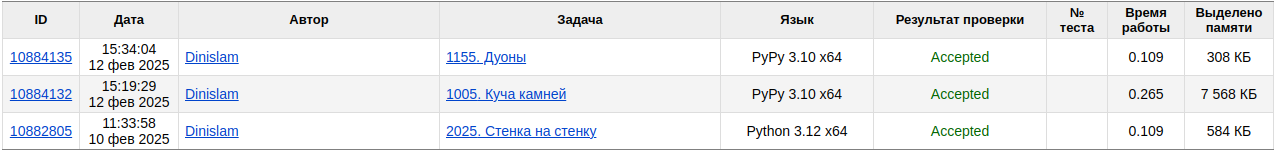
\includegraphics[width=1\textwidth]{check_1.png}
    \caption{Результат проверки}
    \label{fig:compiler-status}
\end{figure}

\end{document}

